\subsection{Data Reduction Studies}
\label{subsec:pmc-results-data-reduction-studies}

This section evaluates the impact of training set size on model performance.
The goal is to determine how many samples are needed to reliably learn the shape-to-memory mapping, especially under the volume-centric assumption.

Experiments progressively subsample the dataset, keeping only the smallest and largest volumes and removing middle-range configurations.
Models used are the same as in prior sections: Gradient Boosting (Envelope), Decision Tree (\ac{GST3D}), and Linear Regression (Gaussian Filter).

\subsubsection{Subsampling Strategy and Motivation}
\label{subsec:data-reduction-strategy-and-motivation}

By excluding central volume values and keeping only extreme configurations, we test how performance degrades with fewer samples.
Figure~\ref{fig:cross_data_reduction_and_residual} shows \ac{RMSE} and residual metrics as the dataset shrinks.

\begin{figure*}[htbp]
    \centering
    \begin{subfigure}[t]{0.49\textwidth}
        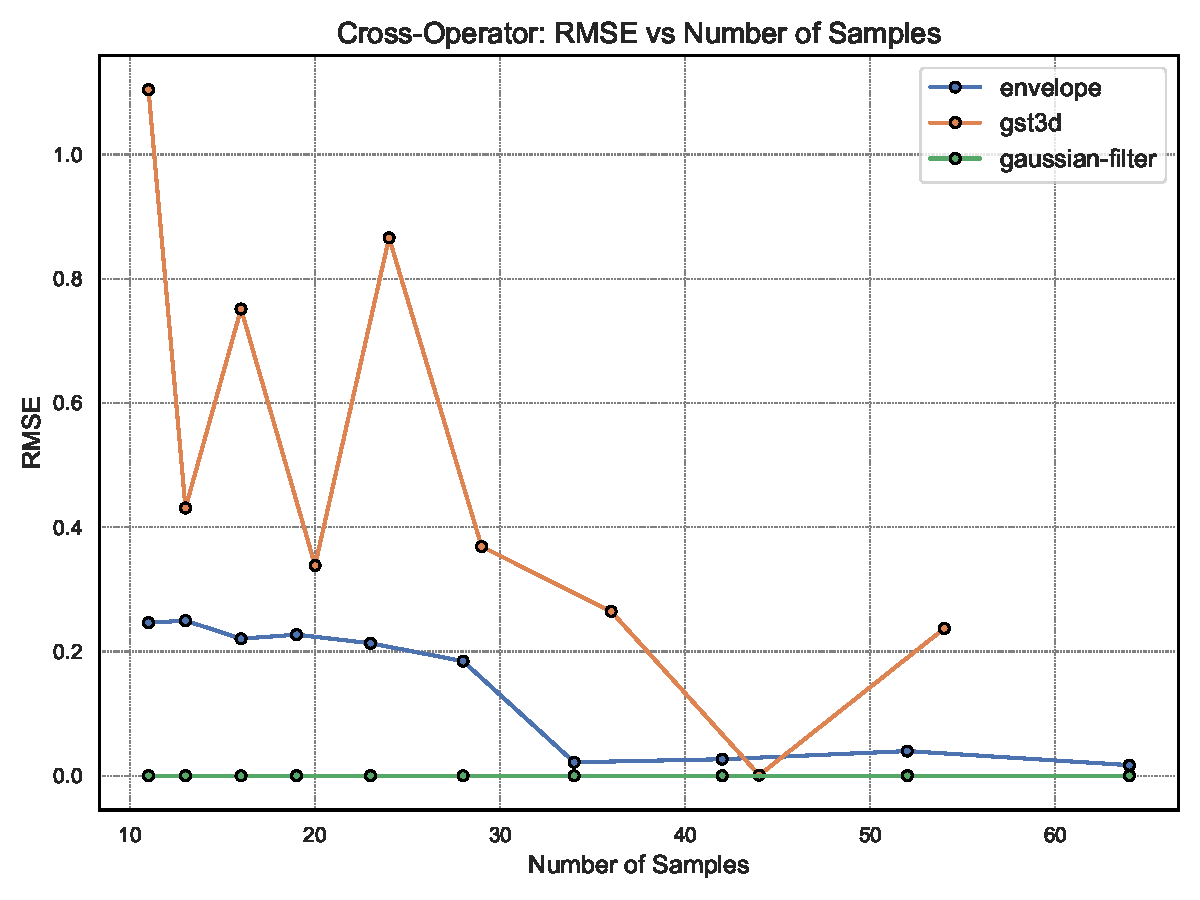
\includegraphics[width=\textwidth]{assets/images/05/cross_data_reduction_rmse}
        \caption{\ac{RMSE} vs. sample size}
    \end{subfigure}
    \hfill
    \begin{subfigure}[t]{0.49\textwidth}
        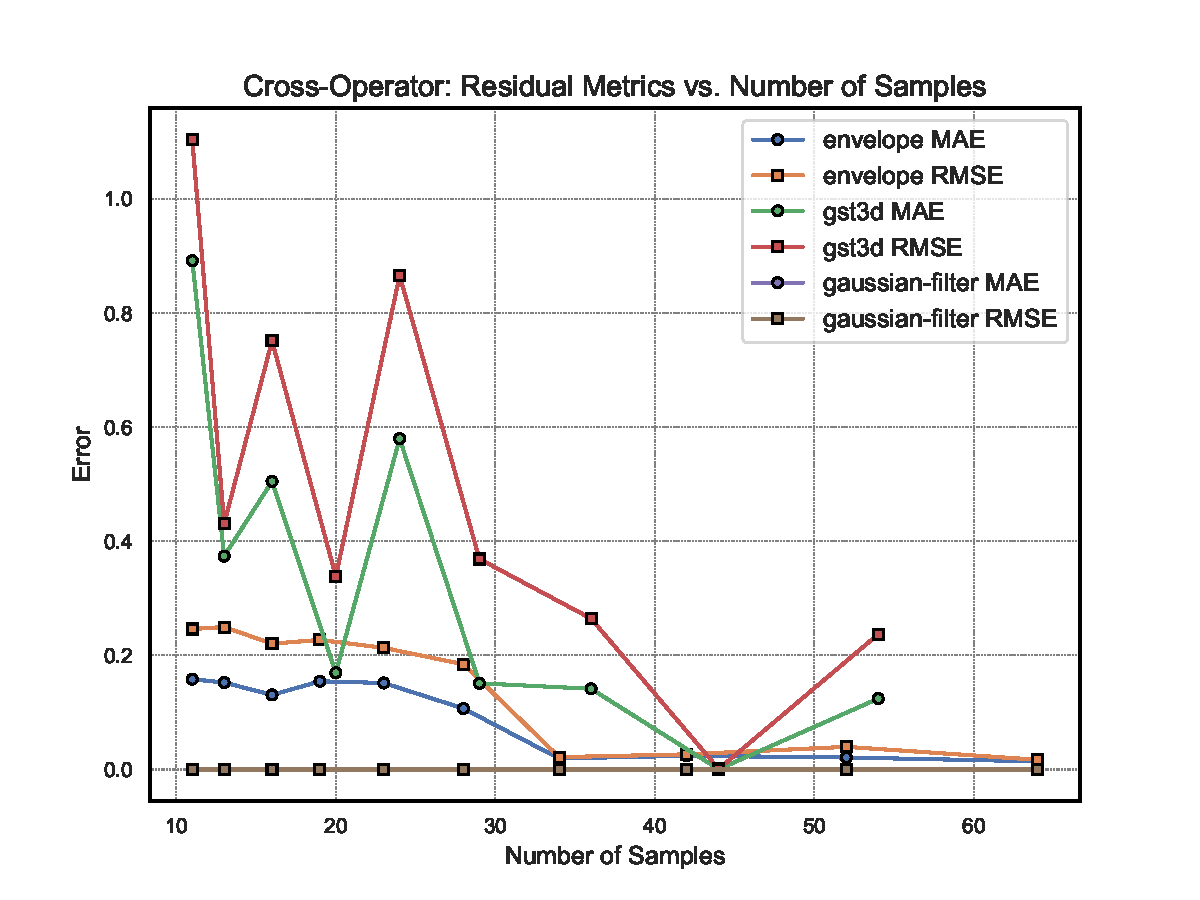
\includegraphics[width=\textwidth]{assets/images/05/residual_metrics_by_sample_size}
        \caption{Residual metrics vs. sample size}
    \end{subfigure}
    \caption{Model performance under data reduction. Moderate pruning preserves accuracy. Severe reduction leads to error spikes.}
    \label{fig:cross_data_reduction_and_residual}
\end{figure*}

\subsubsection{Operator-Wise Performance Trends}
\label{subsec:operator-wise-sample-size-analysis}

Figures~\ref{fig:residual_metrics_by_sample_size_operators} and~\ref{fig:metrics_evolution_sample_size_operators} analyze performance by operator.
Errors grow rapidly below 30 samples, but remain low for 40--50.

\begin{figure*}[htbp]
    \centering
    \begin{subfigure}[t]{0.32\textwidth}
        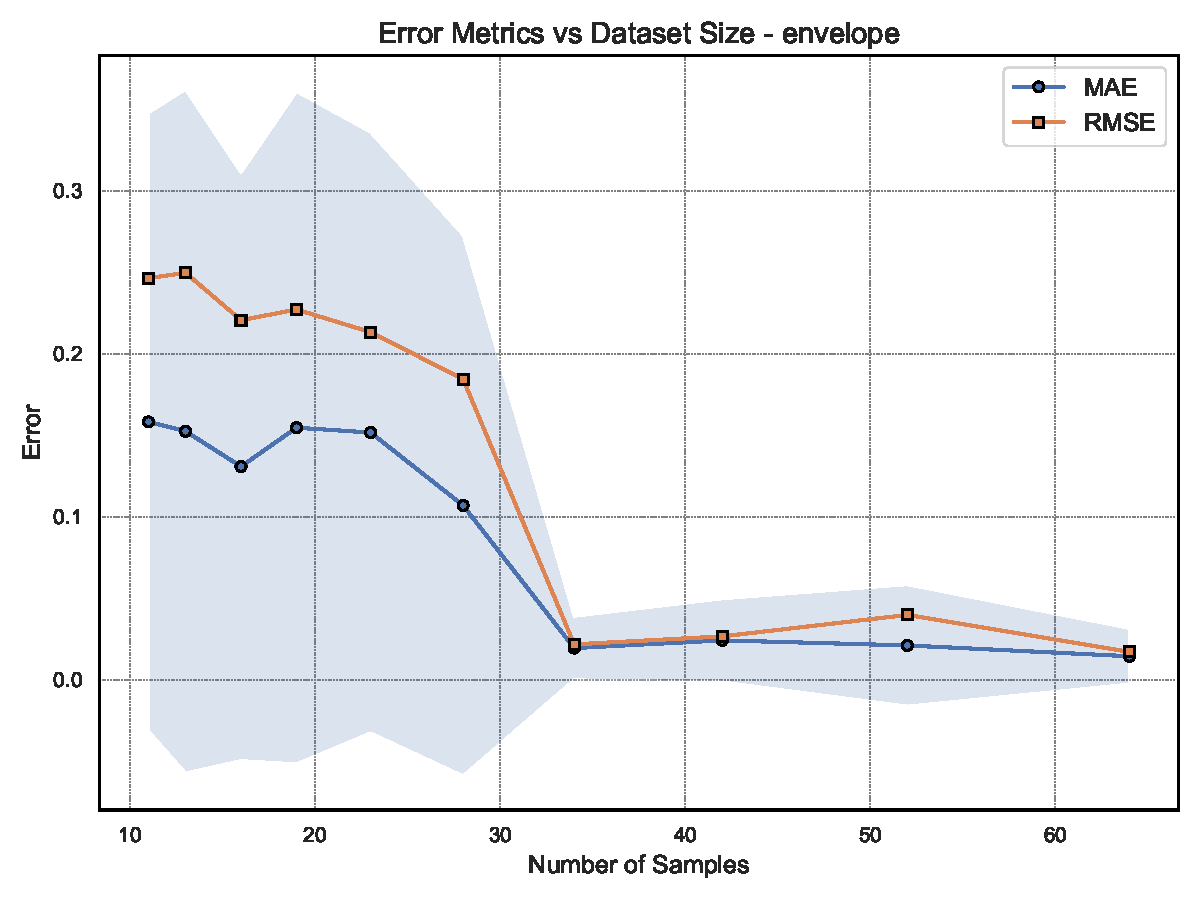
\includegraphics[width=\textwidth]{assets/images/05/residual_metrics_by_sample_size_envelope}
        \caption{Envelope}
    \end{subfigure}
    \hfill
    \begin{subfigure}[t]{0.32\textwidth}
        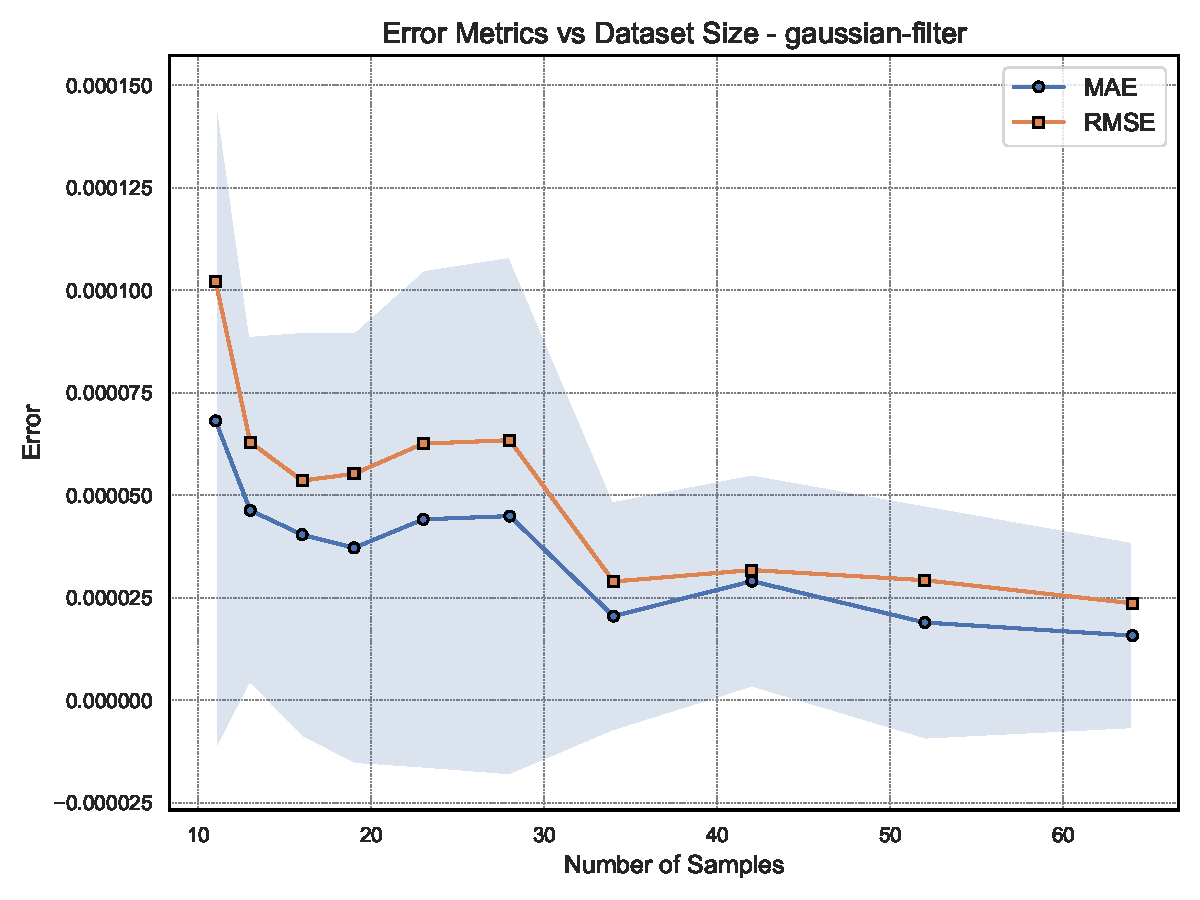
\includegraphics[width=\textwidth]{assets/images/05/residual_metrics_by_sample_size_gaussian-filter}
        \caption{Gaussian Filter}
    \end{subfigure}
    \hfill
    \begin{subfigure}[t]{0.32\textwidth}
        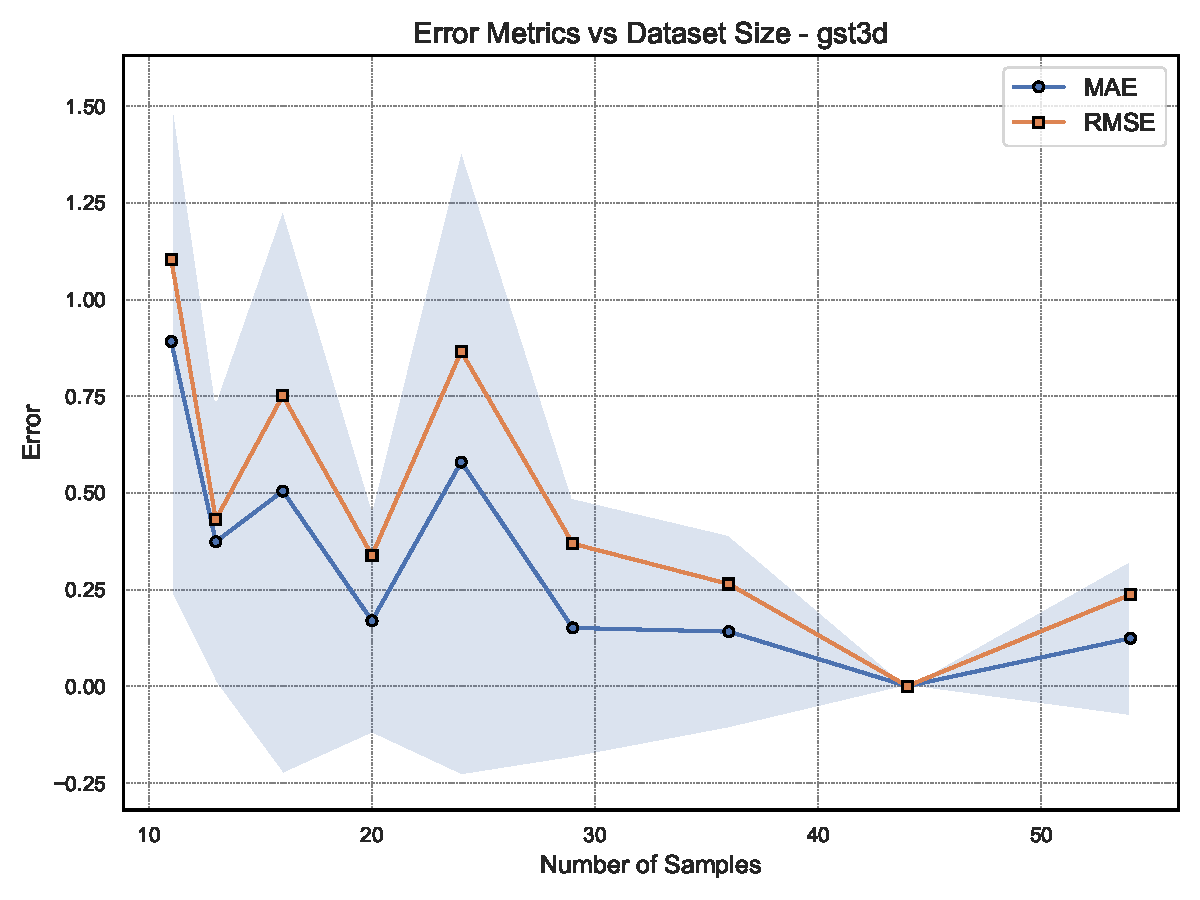
\includegraphics[width=\textwidth]{assets/images/05/residual_metrics_by_sample_size_gst3d}
        \caption{\ac{GST3D}}
    \end{subfigure}
    \caption{Residual metrics by operator. Lower performance below 30 samples.}
    \label{fig:residual_metrics_by_sample_size_operators}
\end{figure*}

\begin{figure*}[htbp]
    \centering
    \begin{subfigure}[t]{0.32\textwidth}
        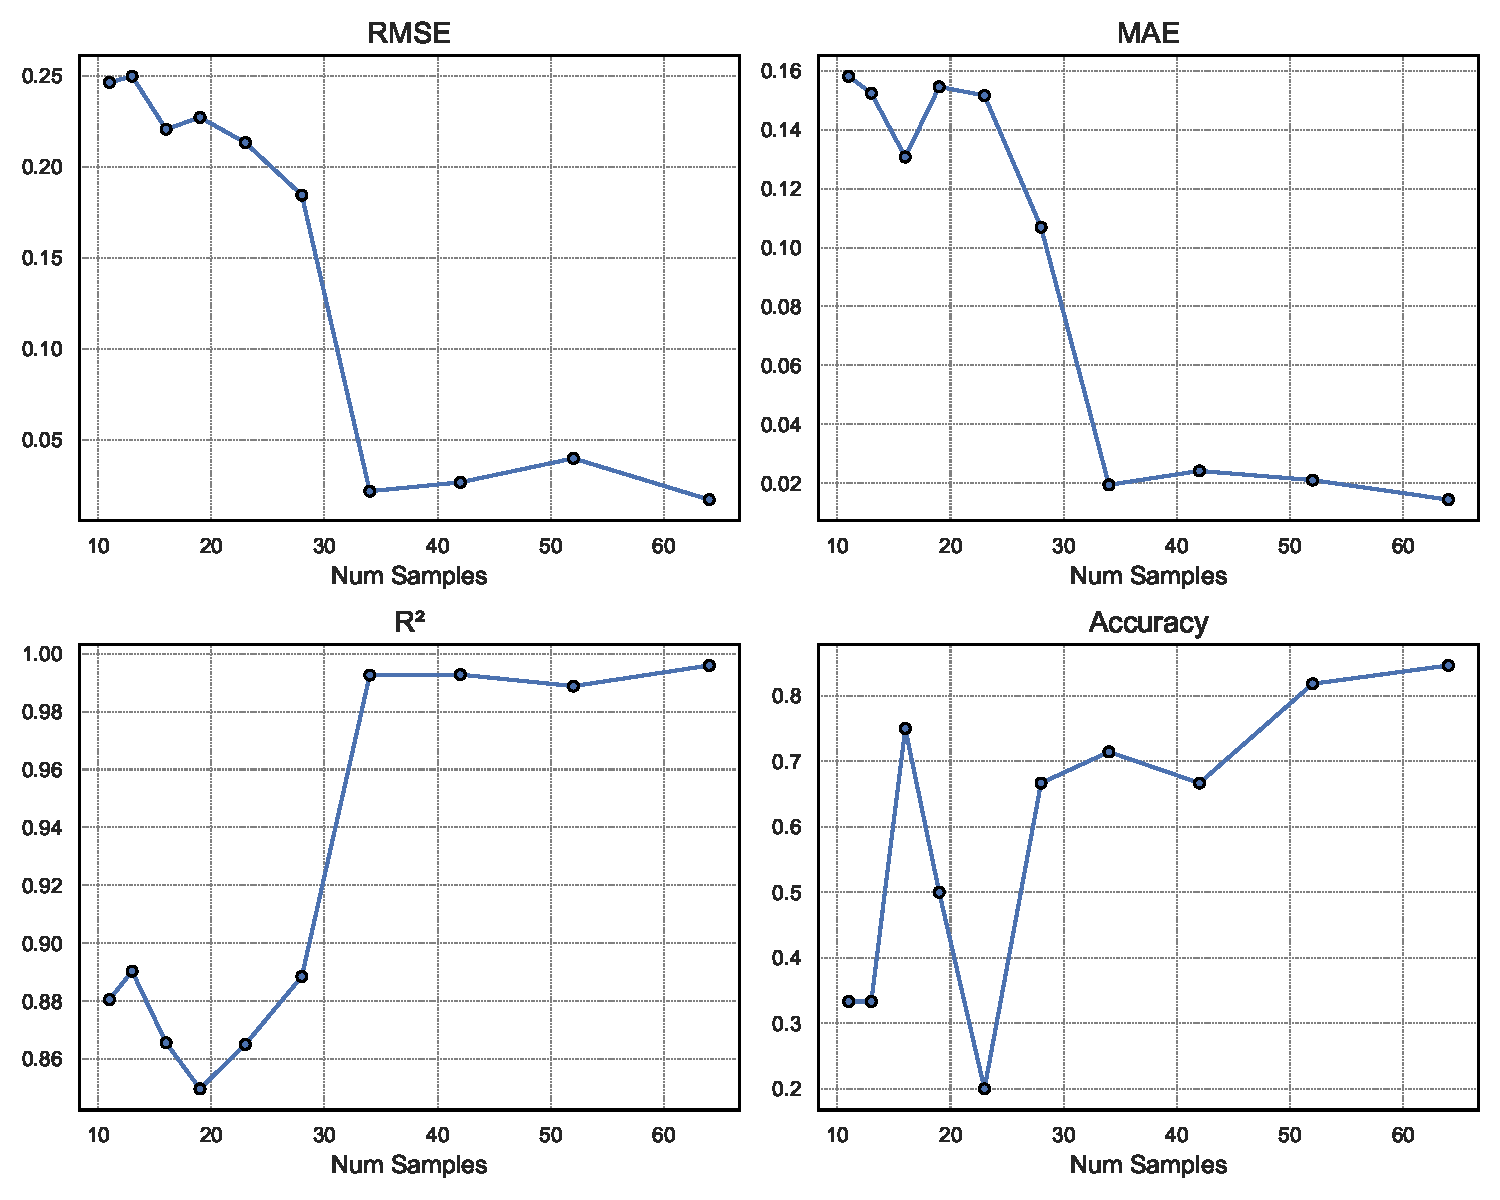
\includegraphics[width=\textwidth]{assets/images/05/metrics_evolution_by_sample_size_envelope}
        \caption{Envelope}
    \end{subfigure}
    \hfill
    \begin{subfigure}[t]{0.32\textwidth}
        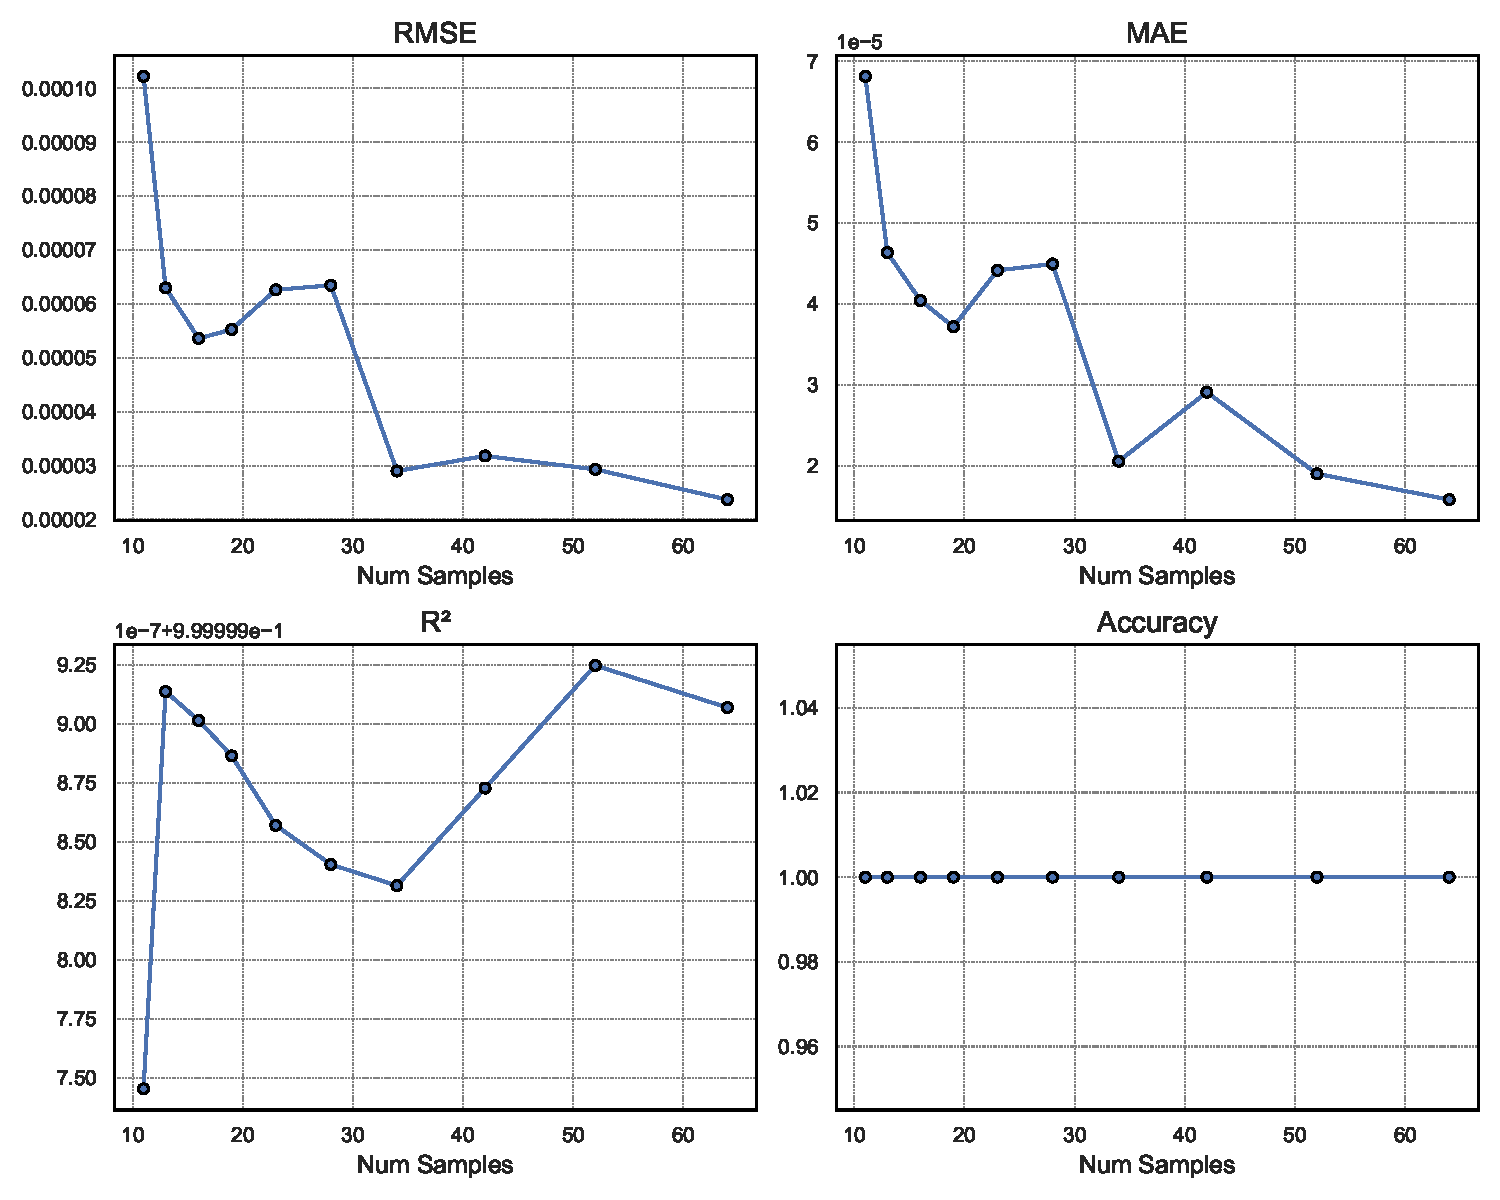
\includegraphics[width=\textwidth]{assets/images/05/metrics_evolution_by_sample_size_gaussian-filter}
        \caption{Gaussian Filter}
    \end{subfigure}
    \hfill
    \begin{subfigure}[t]{0.32\textwidth}
        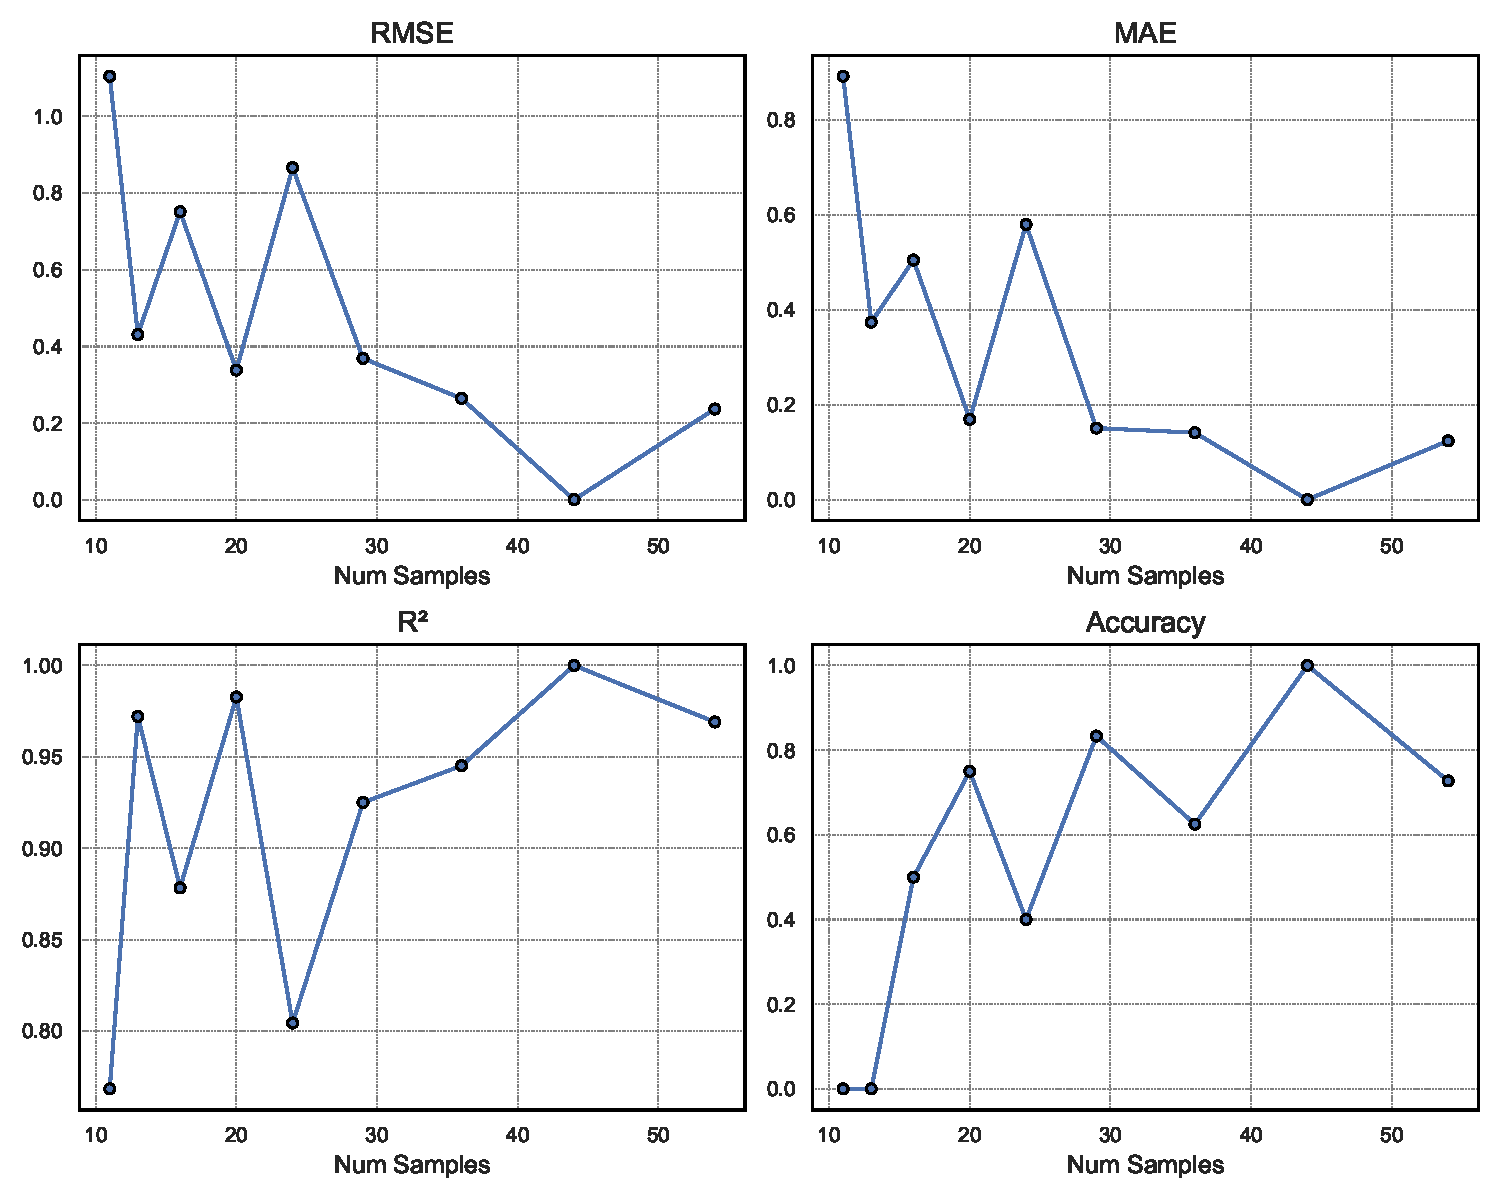
\includegraphics[width=\textwidth]{assets/images/05/metrics_evolution_by_sample_size_gst3d}
        \caption{\ac{GST3D}}
    \end{subfigure}
    \caption{Evolution of \ac{RMSE}, \ac{MAE}, $R^2$, and accuracy as sample size decreases. Performance remains stable down to ~30 samples.}
    \label{fig:metrics_evolution_sample_size_operators}
\end{figure*}

\subsubsection{Score Comparisons and Sweet Spot Around 30 Samples}
\label{subsec:score-comparisons-and-sweet-spot}

Figure~\ref{fig:score_by_sample_size_operators} shows that all operators experience a drop in score when sample count falls below 30--35.
Above that range, model performance saturates and does not improve significantly.

\begin{figure*}[htbp]
    \centering
    \begin{subfigure}[t]{0.32\textwidth}
        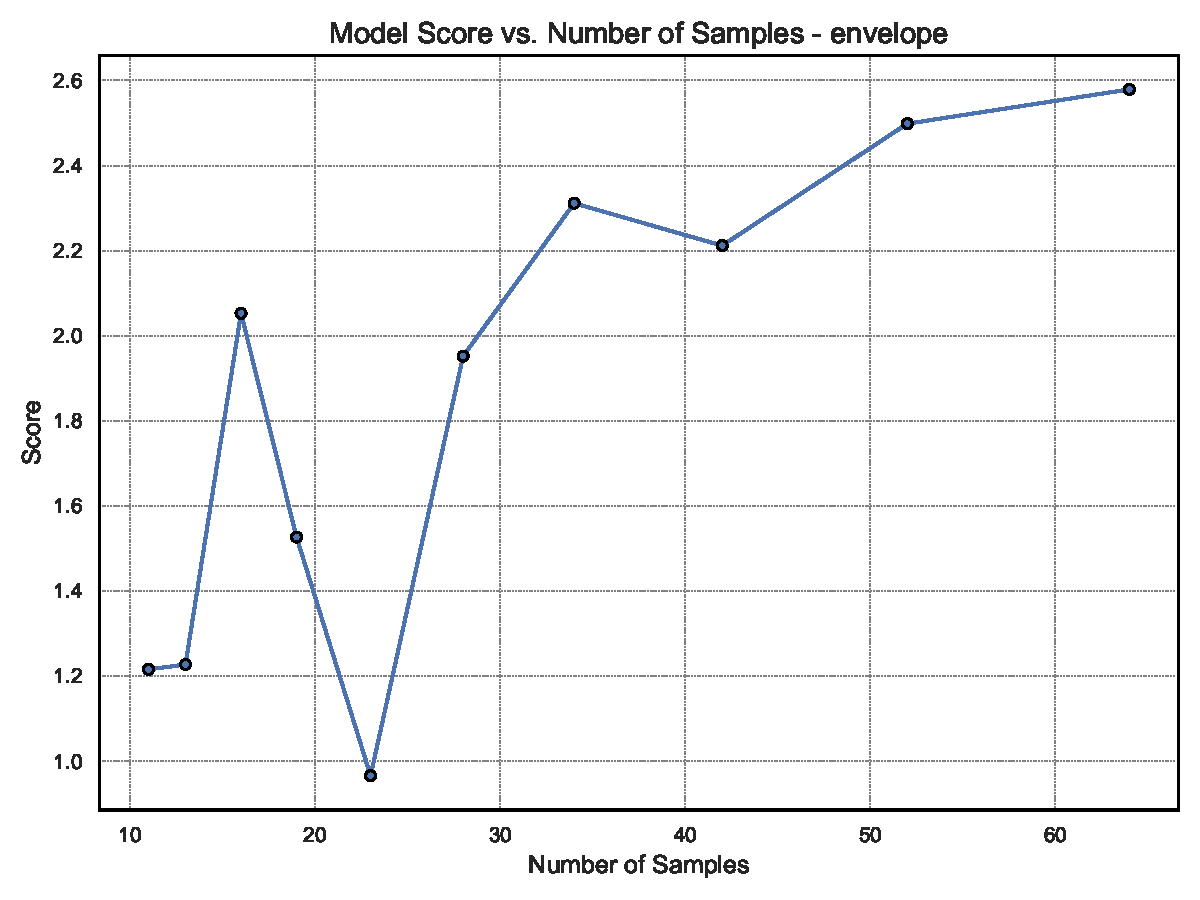
\includegraphics[width=\textwidth]{assets/images/05/score_by_sample_size_envelope}
        \caption{Envelope}
    \end{subfigure}
    \hfill
    \begin{subfigure}[t]{0.32\textwidth}
        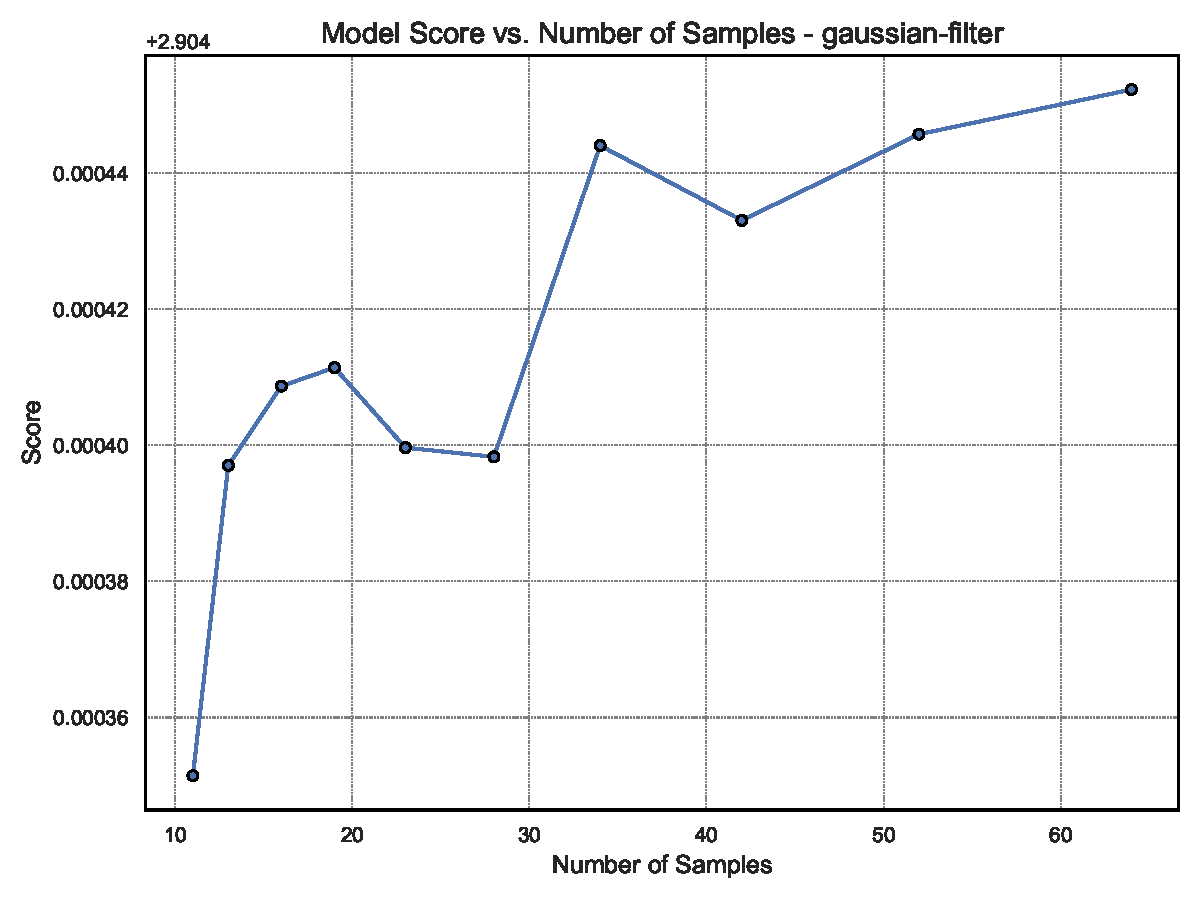
\includegraphics[width=\textwidth]{assets/images/05/score_by_sample_size_gaussian-filter}
        \caption{Gaussian Filter}
    \end{subfigure}
    \hfill
    \begin{subfigure}[t]{0.32\textwidth}
        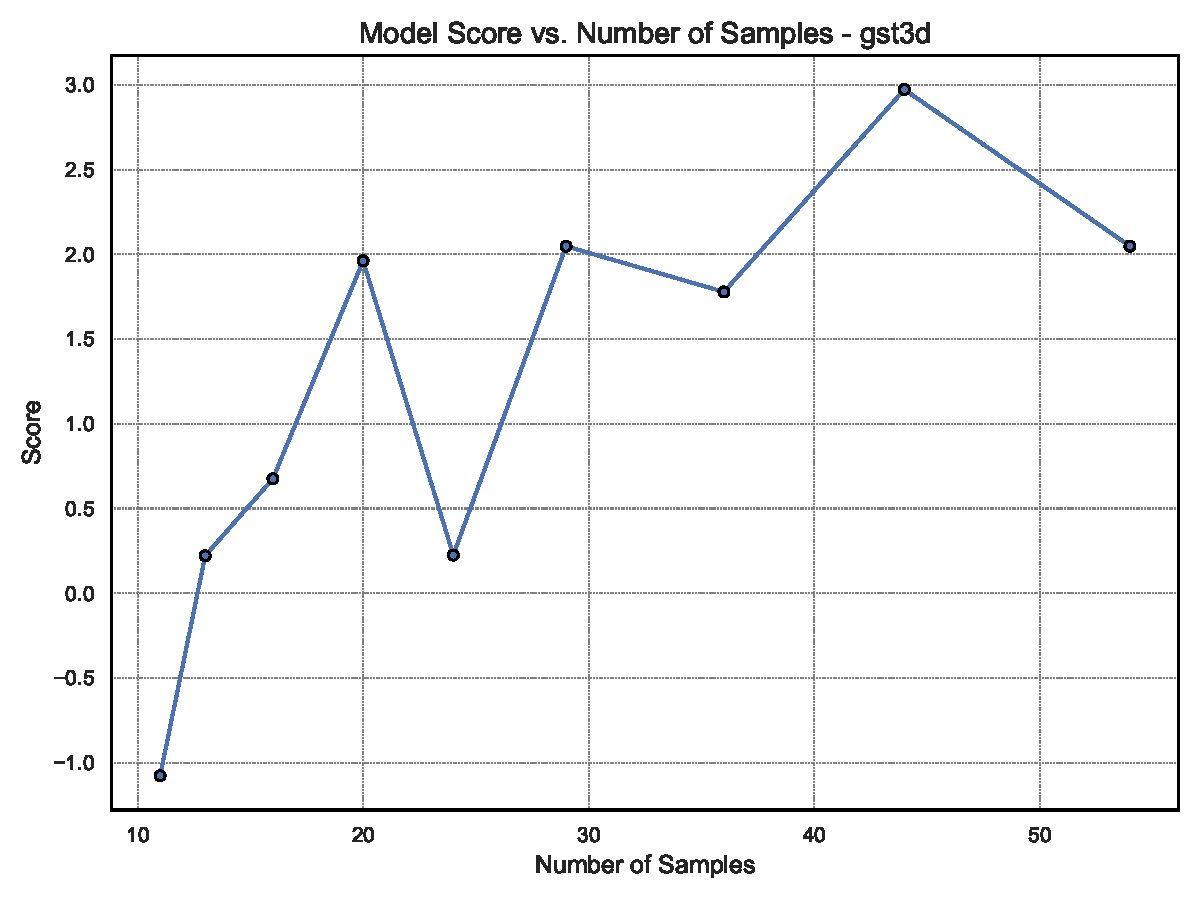
\includegraphics[width=\textwidth]{assets/images/05/score_by_sample_size_gst3d}
        \caption{\ac{GST3D}}
    \end{subfigure}
    \caption{Model score vs. sample count. Scores remain high for $\geq 30$ samples.}
    \label{fig:score_by_sample_size_operators}
\end{figure*}

\begin{table}[htbp]
    \centering
    \begin{tabular}{lccc}
        \hline
        \textbf{Operator} & \textbf{\#Samples} & \textbf{\ac{RMSE}} & \textbf{$R^2$} \\
        \hline
        Envelope          & 64                 & 0.0170             & 0.9959         \\
        Envelope          & 34                 & 0.0217             & 0.9926         \\
        Envelope          & 11                 & 0.2463             & 0.8805         \\
        \ac{GST3D}        & 54                 & 0.2371             & 0.9691         \\
        \ac{GST3D}        & 29                 & 0.3689             & 0.9251         \\
        \ac{GST3D}        & 11                 & 1.1042             & 0.7684         \\
        Gaussian Filter   & 64                 & $2.4\times10^{-5}$ & 0.9999999      \\
        Gaussian Filter   & 34                 & $2.9\times10^{-5}$ & 0.9999998      \\
        Gaussian Filter   & 11                 & $1.0\times10^{-4}$ & 0.9999997      \\
        \hline
    \end{tabular}
    \caption{Selected results from data-reduction study. Performance degrades most notably below 30 samples.}
    \label{tab:data_reduction_summary}
\end{table}

\subsubsection{Conclusions on Data Pruning}
\label{subsec:data-reduction-conclusions}

Model accuracy remains high with only 30--40 samples per operator.
This supports practical deployment of memory estimators using small training datasets.
\ac{GST3D} is more sensitive, while Envelope and Gaussian Filter remain robust with fewer configurations.
Volume extremes provide valuable learning signal, but some middle-volume coverage improves stability.